\documentclass[a4paper,11pt]{article}
\usepackage{fullpage}
\usepackage{hyperref}
\usepackage{url}
\usepackage{graphicx}

\setlength{\parindent}{0pt}
\addtolength{\parskip}{\baselineskip}

\title{3rd Year Group Project\\Report One\\\emph{Inception}}
% \author{Maciej Albin, Rafal Szymanski, Sam Wong, Suhaib Sarmad, Jamal Khan, Suhaib Sarmad}

\author{
    \small{Rafal Szymanski}\\
		\small{\emph{rs2909}}
  	\and
    \small{Maciej Albin}\\
		\small{\emph{mja108}}
    \and
    \small{Sam Wong}\\
		\small{\emph{sw2309}}
    \and
    \small{Suhaib Sarmad}\\
		\small{\emph{sss308}}
		\and
		\small{Jamal Khan}\\
		\small{\emph{jzk109}}
		\and
		Department of Computing - Imperial College London
}


\begin{document} 
	\maketitle
	%\tableofcontents
	%\newpage
	
	\section{Introduction}
	
	\begin{quote}
\emph{In a world where technology exists to enter the human mind through dream invasion, a highly skilled thief is given a final chance at redemption which involves executing his toughest job to date: Inception.}	\end{quote}

	In this group project, we wish to provide an interface to let people see the public Twitter reaction to current events sourced from news RSS feeds.

	
	\section{Key Requirements}
		
		\begin{itemize}
			\item Getting top news stories from Google News RSS Feed
			\item Generating keywords from those news stories, including headlines, and the articles themselves
			\item Getting relevant tweets using the Twitter Streaming API, and giving it the keyword list above
			\item Attaching tweets to appropriate news stories
			\item Generating word clouds for news stories
			\item Fluid live updating UI
		\end{itemize}
		
	\section{Extensions}
	
		\begin{itemize}
			\item Sentiment Analysis of the tweets
			\item Categorisation of tweets into topics
			\item Enriching the news story with other content, such as keyword related pictures
		\end{itemize}
	
	\section{Choice of Development Method}
		\subsection{Development Methods}
		
			We are planning on using agile development methodology with scrum framework. As our development board that has our \emph{product backlog}, and the \emph{current iteration}, we shall be using Trello\footnote{\url{http://trello.com}}.
			\begin{center}
			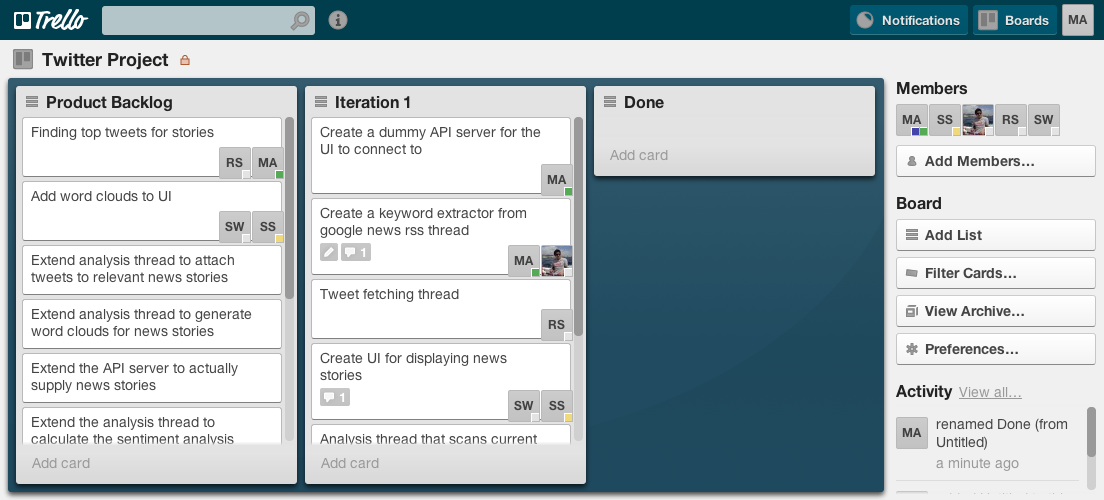
\includegraphics[scale=0.4]{trello.png}
		  \end{center}
	
			The \emph{product backlog} has all the features that we would like to implement. This list will will have items added to it as the project progresses. At the beginning of each week, we shall have a scrum meeting where we pull some required features from the \emph{product backlog} into an \emph{iteration list} that will keep track of what is to be done each week. The Trello software allows us to assign developers to particular tasks, and this feature will be used.
			
			We shall have scrum meetings either daily, or every two days, where we will discuss the progress of the task everyone has been assigned to for that week. We aim to successfully complete the required tasks at the end of each iteration period.
			
			For development itself we will try to utilise \emph{paired programming} as much as possible. We believe this will allow all members of the team to understand major parts of the application in detail and help to even out different levels of expertise between team members. We also believe it will boost the team's productivity.
	
	
		\subsection{Version Control and Code Testing}
		
			We will be using git for version control. Currently the project is hosted on github\footnote{\url{https://github.com/radicality/Twitter-News}}, but we will probably move it soon to our own VPS to set up continuos integration, and instant deployment.
			
			TESTING TO DO
			
			
		\subsection{Needed Information Technology}
			We have decided to use Python as the core programming language, along with MongoDB as the persistent datastore for keeping news and tweet information. MongoDB is particularly useful, as it allows easy saving and retrieval of tweets that come in json format. For the UI we'll be using html5 and javascript.
			
	
	\section{Draft Schedule}
	
		We are currently in Week 4 of the term, and the project is to be handed in by 10th December, ie the end of week 10.
		
		Our progression plan is as follows:
		
		\begin{itemize}
			\item By end of Week 4:
			\item By end of Week 5: 
			\item By end of Week 6: 
			\item By end of Week 7: 
			\item By end of Week 8: 
			\item By end of Week 9: 
			\item By end of Week 10:
		\end{itemize}
	
	\section{Detailed Plan for First Iteration}
	\begin{itemize}
	  \item Create Dummy API server for the UI to connect to and define API calls
	  \item Basic UI for displaying news stories
	  \item Create a tweet fetching and analysis process:
	  \begin{itemize}
	    \item Thread to extract keywords from google news stories
	    \item Thread to fetch tweets based on keywords
	    \item Thread to assign tweets to news stories
	  \end{itemize}
	  \item Setup continuos integration
	\end{itemize}
		

\end{document}